\documentclass[crop, tikz]{standalone}
\usepackage{tikz}

\usetikzlibrary{positioning}

\begin{document}
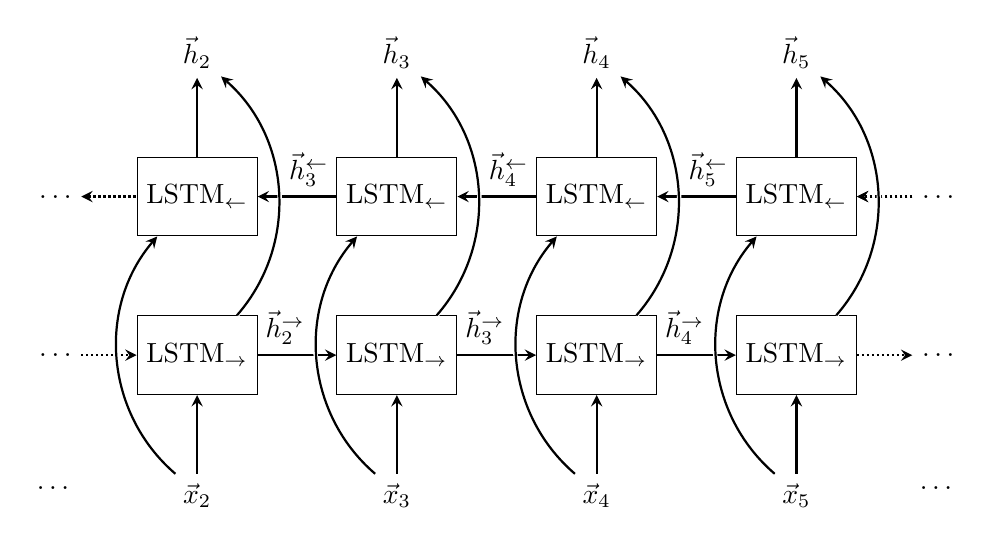
\begin{tikzpicture}
	\node[rectangle] (Y0) at (0, 0) {$\dots$};
	\node[rectangle, draw, right=2em of Y0, minimum height=1cm, minimum width=1cm] (RNN) {LSTM$_\rightarrow$};
	\node[rectangle, right=of RNN, draw, minimum height=1cm, minimum width=1cm] (RNN2) {LSTM$_\rightarrow$};
	\node[rectangle, right=of RNN2, draw, minimum height=1cm, minimum width=1cm] (RNN3) {LSTM$_\rightarrow$};
			
	\node[rectangle, right= of RNN3, draw, minimum height=1cm, minimum width=1cm] (RNN4) {LSTM$_\rightarrow$};
	\node[rectangle, right=2em of RNN4] (RNN5) {$\dots$};
			
			
	\node[rectangle, above=of RNN4, draw, minimum height=1cm, minimum width=1cm] (R25) {LSTM$_\leftarrow$};
	\node[rectangle, left=of R25, minimum height=1cm, minimum width=1cm, draw] (R24) {LSTM$_\leftarrow$};
	\node[rectangle, left=of R24, draw, minimum height=1cm, minimum width=1cm] (R23) {LSTM$_\leftarrow$};
	\node[rectangle, left=of R23, draw, minimum height=1cm, minimum width=1cm] (R22) {LSTM$_\leftarrow$};
	\node[rectangle, left=2em of R22] (R21) {$\dots$};
	\node[right=2em of R25] (Y20) {$\dots$};
			
	\node[below=of RNN] (X1) {$\vec{x}_2$};
	\node[below=of RNN2] (X2) {$\vec{x}_3$};
	\node[below=of RNN3] (X3) {$\vec{x}_4$};
	\node[below=of RNN4] (X4) {$\vec{x}_5$};
	\node[above=of R25] (Y5) {$\vec{h}_5$};
	\node[above=of R24] (Y4) {$\vec{h}_4$};
	\node[above=of R23] (Y3) {$\vec{h}_3$};
	\node[above=of R22] (Y2) {$\vec{h}_2$};
			
	\draw[-stealth, thick] (X1) -- (RNN);
	\draw[-stealth, thick] (X2) -- (RNN2);
	\draw[-stealth, thick] (X3) -- (RNN3);
	\draw[-stealth, thick] (X4) -- (RNN4);
	\draw[-stealth, thick, densely dotted] (Y0) -- (RNN);
	\draw[-stealth, thick] (RNN) -- node[above, pos=0.35] {$\vec{h}_2^\rightarrow$} (RNN2);
	\draw[-stealth, thick] (RNN2) -- node[above, pos=0.35] {$\vec{h}_3^\rightarrow$} (RNN3);
	\draw[-stealth, thick] (RNN3) -- node[above, pos=0.35] {$\vec{h}_4^\rightarrow$} (RNN4);
	\draw[-stealth, densely dotted, thick] (RNN4) -- (RNN5);
	\node[below=4em of Y0] (d) {\dots};
	\node[below=4em of RNN5] (d) {\dots};
			
	\path[-stealth, ultra thick, white] (X1) edge[bend left=45] (R22);
	\path[-stealth, thick] (X1) edge[bend left=45] (R22);
	\path[-stealth, ultra thick, white] (X2) edge[bend left=45] (R23);
	\path[-stealth, thick] (X2) edge[bend left=45] (R23);
	\path[-stealth, ultra thick, white] (X3) edge[bend left=45] (R24);
	\path[-stealth, thick] (X3) edge[bend left=45] (R24);
	\path[-stealth, ultra thick, white] (X4) edge[bend left=45] (R25);
	\path[-stealth, thick] (X4) edge[bend left=45] (R25);
	\draw[-stealth, densely dotted, thick] (Y20) -- (R25);
			
	\draw[-stealth, thick] (R22) -- (Y2);
	\draw[-stealth, thick] (R23) -- (Y3);
	\draw[-stealth, thick] (R24) -- (Y4);
	\draw[-stealth, thick] (R25) -- (Y5);
		
	\draw[stealth-, densely dotted, thick] (R21) -- (R22);
	\draw[stealth-, thick] (R22) -- node[above, pos=0.65] {$\vec{h}_3^\leftarrow$} (R23);
	\draw[stealth-, thick] (R23) -- node[above, pos=0.65] {$\vec{h}_4^\leftarrow$} (R24);
	\draw[stealth-, thick] (R24) -- node[above, pos=0.65] {$\vec{h}_5^\leftarrow$} (R25);
	\draw[-stealth, densely dotted, thick] (Y20) -- (R25);	
			
	\path[-stealth, ultra thick, white] (RNN) edge[bend right=45] (Y2);
	\path[-stealth, thick] (RNN) edge[bend right=45] (Y2);
	\path[-stealth, ultra thick, white] (RNN2) edge[bend right=45] (Y3);
	\path[-stealth, thick] (RNN2) edge[bend right=45] (Y3);
	\path[-stealth, ultra thick, white] (RNN3) edge[bend right=45] (Y4);
	\path[-stealth, thick] (RNN3) edge[bend right=45] (Y4);
	\path[-stealth, ultra thick, white] (RNN4) edge[bend right=45] (Y5);
	\path[-stealth, thick] (RNN4) edge[bend right=45] (Y5);
			
\end{tikzpicture}
\end{document}
